\documentclass{article}
\usepackage[utf8]{inputenc}
\usepackage{hyperref}
\hypersetup{
colorlinks=true,
    linkcolor=black,
    filecolor=black,      
    urlcolor=blue,
    citecolor=black,
}
\usepackage[letterpaper, portrait, margin=1in]{geometry}
\usepackage{enumitem}
\usepackage{amsmath}
\usepackage{booktabs}
\usepackage{graphicx}
\usepackage{titlesec}

\titleformat{\section}
{\normalfont\Large\bfseries}{\thesection}{1em}{}[{\titlerule[0.8pt]}]
  
\title{Homework 4 \\ Economics 7103}
\author{Ana Mazmishvili}
\date{February 12}
  
\begin{document}
  
\maketitle

\section{Python}

\noindent 1. See figure \ref{fig:trend}

\begin{figure}[h]
    \centering
    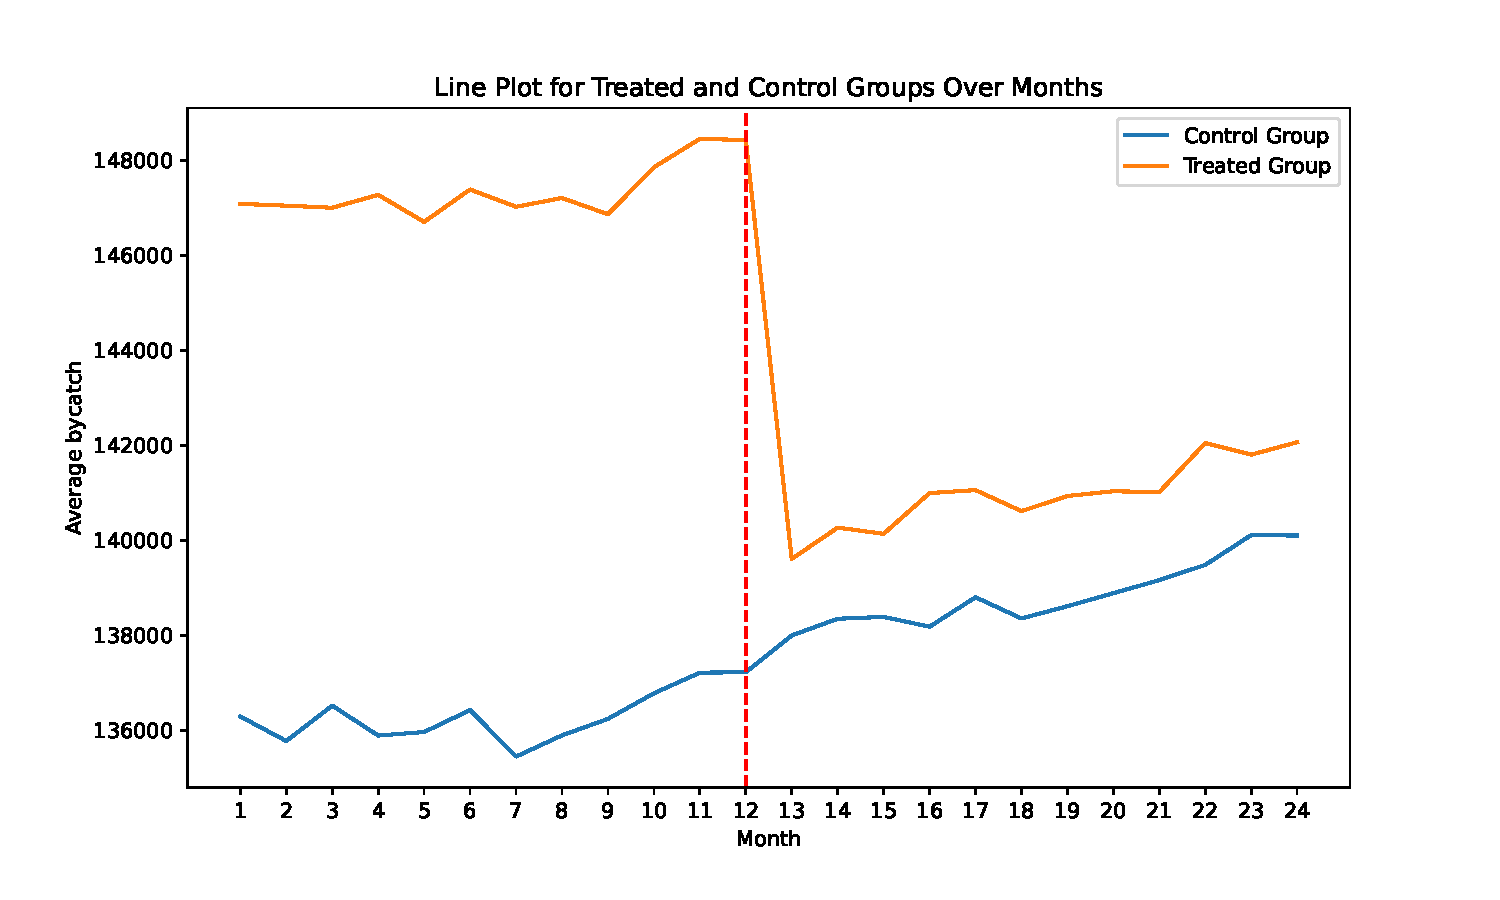
\includegraphics{homework 4/output/figure/trend1.pdf}
    \caption{ Bycatch by month before and after treatment. }
    \label{fig:trend}
\end{figure}

\noindent 2. See table \ref{tab:DID1}

\begin{table}[]
    \centering
    const             136310.169457
treated            11052.449649
post_treatment      2563.075526
trt_posttrt        -8956.783746
dtype: float64

    \caption{DID results}
    \label{tab:DID1}
\end{table}


\noindent 3. Each method produces quite similar results that probably only differ in rounding error:

\noindent 4. See table .  If randomization worked, the simple difference-in-means is an unbiased estimate of the treatment effect.
\section{Stata}

\noindent 1. See table 



\noindent 2. See figure 



\noindent 3. See table 



\end{document}